% !TEX root = ../main.tex
% !TEX program = XeLaTeX
% !TEX encoding = UTF-8 Unicode

\date{2018년 3월 7일}

\begin{frontmatter}
\title{빠꼬어}
\author{김성}
\address{한국외국어대학교 베트남어과}
\begin{abstract}
Alves, Mark J. (2006). A grammar of Pacoh: a Mon-Khmer language of the central highlands of Vietnam. Pacific Linguistics, Research School of Pacific and Asian Studies, The Australian National University, 1--26.
\end{abstract}
\end{frontmatter}

%%%%%

\section*{발제 범위 분배}
\begin{table}[h]
\begin{center}
\def\arraystretch{1.5}
\begin{tabular}{>{\sffamily}ccccl}
\hline
	&\itshape 발제자	&\itshape 발제 범위		
	&\itshape 페이지	&\itshape 내용\\
\hline
1 & 김성 & Ch. 1-2 & pp. 1-26 & 서론, 음운론 \\
2 & & Ch. 3-6 & pp. 27-53 & 형태론, 기본 구 구조 개괄, 부사, 접속사 \\
3 & & Ch. 7 & pp. 54-78 & 명사 \\
4 & & Ch. 8-10 & pp. 79-105 & 전치사, 문장 소사, 기본 동사 \\
5 & & Ch. 11 & pp. 106-111 & 보조 동사, SVC, VCT 동사 \\
\hline
\end{tabular}
\end{center}
\end{table}

\section{서론}
베트남 트어 티엔/후에 성과 꽝찌 성의 중부 고지대에서 주로 사용되는 빠꼬어의 기술 문법.

\subsection{본 문법서의 목적과 쓰임}
\begin{itemize}
\item 빠꼬어를 포함한 몬·크메르어파 언어에 대한 후속 연구를 위한 정확한 데이터 제공
\item 몬·크메르어의 전형적인 특징들에 대한 분석적 접근
\item 비교·유형론적 관점에서 빠꼬어와 다른 몬·크메르어에서 공통적으로 보이는 문법적 특징을 기술
\end{itemize}

\subsection{언어 계통론과 몬·크메르어의 유형론적 특성}
\begin{itemize}
\item 빠꼬어는 몬·크메르어파에서 Katuic(중부 베트남, 남부 라오스, 북동부 태국 일부) 하위계통(subbranch)에 속함. 몬·크메르어파는 동남아와 인도 동부에 퍼져 있는 남아어족(Austroasiatic)의 일파.

\item 빠꼬어는 몬·크메르어파의 다른 하위계통 언어들과 언어 구조, 23\%~30\% 정도의 핵심어휘를 공유함. 다른 하위계통 언어들 사이의 비율과 비슷한 수준.

\item 빠꼬어가 갖는 몬·크메르어파 (및 일부 다른 동남아 언어)의 유형론적인 특징
\begin{center}
\begin{tabular}{lp{.7\linewidth}}
\hline
\textbf{문장 구조}& 주-술 구조. SVO.\\
\textbf{명사구 구조}& 종별사 언어, 명사 - 수식어 어순, 어휘적으로 나타나는 복수성 (접사가 아닌)\\
\textbf{modal aspects}& 시제와 의문형이 문장 소사(particle)이 아니라 부사로 나타남. (동사 활용이나 접사가 아닌)\\
\textbf{단어 형성}& (사역동사 등을 만드는) 전음절이나 (동사에서 파생된 명사 등을 만드는) 접요사, 부분적(교체적) 반복어\\
\textbf{음운론적 단어 구조}& 1.5음절 단어 구조. 전음절은 강세를 받지 않고 형태 상 약간 축소. 주음절에 자음군.\\
\textbf{음운론}& 모음에서 나타나는 register 차이, 조음 위치 4가지(순음, 치음, 경구개음, 연구개음)\\
\hline
\end{tabular}
\end{center}
\end{itemize}

\subsection{빠꼬어의 언어적 상황과 사회언어학적 문제}
빠꼬어는 베트남 중부 고지대 일부 지역의 소수민족이 사용하는 언어이다. 정확한 수는 확인하기 어렵지만 화자 수는 10,000명을 넘는다. 베트남의 공식 소수민족 목록에는 빠꼬 족이 포함되지 않았다. 빠꼬 족에 가까운 따오이(Taoih)족이 포함되어 있으나 따오이어와 빠꼬어는 어휘적으로도 음운론적으로도 명백히 서로 다른 언어이다. 아 르어이(A-Lưới) 계곡이 문화적 중심지이지만 트어 티엔 성과 꽝 찌 성 내의 다른 지역에서도 빠꼬어는 사용된다.

빠꼬인들은 전통적으로 화전을 일구거나 무기 및 덫으로 사냥을 하고 살았으나 지금은 저임금 수공업 등으로 생활 방식이 바뀌고 있다. 젊은 세대는 농업이나 사냥에 대한 지식을 잃어 가고 있다. 그에 따라 관련된 어휘나 음운론, 형태론, 통사론적인 패턴이 함께 사라져 가고 있다. 또 학교에서 빠꼬 인들이 베트남어를 점점 더 많이 사용하고 고지로 이주하는 베트남인이 많아짐에 따라 이미 빠꼬어에 유입되어 있는 베트남어 문법 (e.g. 사역형 형태소를 사용하는 대신 '주다'와 '하다' 동사를 사용하여 사역 형태를 만드는 일이 많아짐)이나 관련된 어휘들 (e.g. {\itshape{là}} ‘~이다’, {\itshape{bằng}} ‘~으로’ 등)의 사용이 점점 더 많아질 것으로 예상된다. 결정적으로 빠꼬어 대신 베트남어를 사용하도록 만드는 사회적, 경제적, 정치적 압력이 상당하다.

\subsection{선행 연구와 데이터 수집}
선행 연구자들에게 받은 카세트 테이프와 전사 기록, 본인이 직접 1997, 1998년에 원어민에게서 채록.
참고

\subsection{데이터 분석과 개념}
\begin{itemize} 
\item 형태론에 대해 기저형이나 변형을 상정하지 않음.

%먼가.. 독특한 개념을 많이 만들어 놓은 것 같으니 음운론에 표를 먼저 넣고 내용을 다 정리한 다음에 시간이 나면 더 넣자
\item 이 문법서에서 독특하게 가정하고 있는 점 3가지
\begin{enumerate}
\item (의미론과 의미론에 관련된 요소는 중요하지만) 통사론은 표층의 한 층위(one level of representation)에서 설명된다.
\item 발화된 단어가 통사구조의 통사적 중심이다.
\item 동음이의어(homophony)가 눈에 보이는 분포적 변이에 대해 많은 것을 설명한다.
\end{enumerate}

많이 바뀌고 있고 정확하지 않을 수 있으니 주의하라.
\end{itemize}

\section{음운론}
\begin{itemize} 
\item 빠꼬어의 음운론은 몬·크메르어파의 다른 언어와 대부분 유사하다.
\item Register와 장단 구분에 의해 모음의 개수가 많다. 
\item 자음은 순음, 치경음, 경구개음, 연구개음, 성문음의 다섯 가지 조음위치를 나타낸다. 
\item 1.5음절 단어의 구성이 나타난다. 
\item 이외에 억양, 중첩 형태음운론 등을 살펴본다. 
\end{itemize}

\subsection{전사 체계}
\begin{itemize} 
\item 빠꼬어는 공식 문자체계를 갖추고 있지 않다. IPA 기반 체계와 Quoc Ngu 기반 체계가 있는데, 여기서는 IPA기반으로 전사한다. 자음은 명확하나 모음에는 주의가 필요하다.
\end{itemize}

\subsection{자음}
\begin{itemize}
\item 빠꼬어의 23개 자음 음소는 다음과 같다.
\begin{center}
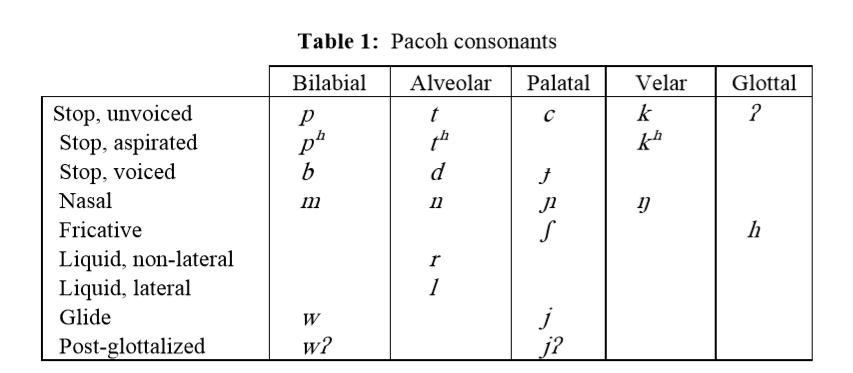
\includegraphics[width=.8\linewidth]{Pacoh/src/Pacohconsonants.png}
\end{center}
\item Watson(1964)에서는 18개로 분석했으나 여기서는 유기 폐쇄음 3개와 후-성문음화(post-glottalized)된 유음 2개를 추가하였다. (Alves (2000) 참조)

\item 베트남어 차용어에만 나타나는 음소는 넣지 않았다.
\end{itemize}

\subsubsection{자음 종류(classes)}
\begin{itemize}
\item 빠꼬어 무성 파열음의 분포는 다음과 같다.
\begin{enumerate}
\item 음절초와 음절말에 모두 나타난다.
\item 전음절(presyllables)에서는 onset 이다.
\item 음절 말에서는 불파음이다.
\end{enumerate}
\item /p, t, k/는 모든 위치에서 가장 높은 빈도로 나타난다. 이 소리가 들어간 단어 초의 접사가 2음절 단어에서 자주 나타나는 것이 가장 큰 이유이다. 1음절 단어에서는 다른 음소와 분포상 큰 차이가 없다.
\item 후-성문음화된 활음은 음절말에만 나타난다.
\end{itemize}

\paragraph{성문 파열음}
\begin{itemize}
\item 성문 파열음은 빠꼬어에서 변별적인 음소로서 기능한다. 
\item 단어 말 위치에서 성문 파열음이 예측되지 못하는 최소대립쌍이 존재한다. 따라서 음절 정점(peak)은 음절 초 자음 없이는 나타나지 않는다. 
\item 성문 파열음은 단어 내 음절과 음절 사이 위치에서도 명확히 변별적이다. 
\item 성문 파열음은 빠꼬어 음절에 대해 음절초 자음이 있어야 한다는 전반적인 요구를 충족시킨다. (Quoc Ngu 기반 전사 체계에서는 이를 충분히 표현해 내지 못한다.)
\item 발화 연속체에서 음절말 자음은 다음 단어의 모음과 재음절화(resyllabify)하지 않는다. 즉 음절화 이전 음운론적 형태(representation)에 성문 파열음이 있음을 시사하는 것이다.
\item 따라서 음성학적으로도 음소적으로도 모든 빠꼬어 음절에는 첫 자음이 있어야 하고 거기에는 성문 파열음도 포함된다. 이와 유사하게 문장에서는 성문 파열음이 음성학적 변화를 막는다.
\end{itemize}

\paragraph{경구개 마찰음}
\begin{itemize}
\item 경구개 마찰음을 선행 연구와 다르게 상정한 이유. \omission
\end{itemize}

\paragraph{후-성문음화된 활음(post-glottalized glides)}
\begin{itemize}
\item 후-성문음화된 활음에 대해 분절음 군을 상정하면 CCV:C 라는 음절 형태에 맞지 않는다.
\item 다른 동계어에도 이러한 소리가 나타난다.
\item 음소 체계의 균형도 맞지 않는다.
\item 유형론적으로도 유성음과의 대응으로 보는 것보다 저자처럼 하는 것이 자연스럽다.
\item 역사언어학적인 근거도 있다.
\end{itemize}

\subsubsection{조건적인 변화}
\paragraph{음절말 /\textipa{S}/ 앞의 모음 경과음(off-glide) 구개음화} 
/ʃ/의 음성적 실현음은 [ʃ], [jh], [\r{\j}](원문에는 무성음 표시 하얀 원이 없음) 등이다. 마지막 두 경우는 /ʃ/ 폐쇄가 약화되어 나타난 결과.

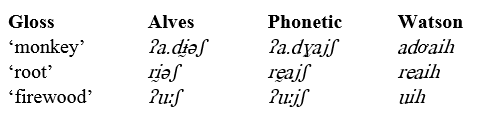
\includegraphics{Pacoh/src/sh-gloss.png}

(Watson 전사에서는 'ih'이지만 음운론적으로는 /i/가 없다고 보는 것이 타당하다는 뜻인 듯)

\paragraph{단어 초의 경음화(fortition)}
마찰음화(spirantization), 삽입음(epenthesis).
\begin{itemize}
\item 마찰음화 : 음절초 /w/ 는 대부분 [v]로 실현, 따라서 선행 연구와 다르게 [v]를 /w/의 변이음으로 봄. 단어 초의 경음화 (labial fortition), 음절 가장자리 (edge)인 음절초 위치에서 공명성이 더 낮은 [v]로 실현.
\item 삽입음 : 주음절 전의 공명음, 즉 비음이나 유음(nasal or liquid presyllables) 앞에는 음운적으로 변별적이지 않은 성문 폐쇄음이 요구됨. 옳지 않은 음절화 방지. 2.2.1.1 참조. 비음은 모음과 같이 공명음이므로 비-공명음인 성문 폐쇄음이 음절의 형태를 최대화함. 비-공명 폐쇄음 중 음소적으로 변별적이지 않은 성문 폐쇄음이 삽입되는 것은 자연스러운 일. 가장 덜 변별적이고 가장 공명성을 덜 갖춘 자음이기 때문이다.
\end{itemize}

\paragraph{음절말 원순음화}
/ŋ/ 와 /k/ 는 [-RTR] (RTR=‘Retracted Tongue Root’) /o/, /u/ 뒤에서 [ŋʷ] [kʷ]로 실현된다. (이유는 명확하지 않지만 [+RTR]인 모음 뒤에서는 원순음화가 일어나지 않는다.) 따라서 [duŋ] ‘house’ 는 음성적으로 [duŋʷ]으로 실현될 수 있다. 모음의 원순성이 자음의 순음화를 유도하는 경향이 있다. 그러나 이 과정이 늘 나타나는 것은 아니고 발화의 속도나 명확성에 따라 차이를 보인다. 완전히 [m]으로 추이되는 것은 용납되지 않는다. 이러한 경향성은 베트남어의 동일한 음성적 환경에서 나타나는 규칙적 원순음화와 궤를 같이하며 어쩌면 지역적인 경향성일지 모른다.

\subsubsection{전음절(presyllable)에서의 비음 동화}
전음절의 비음이 후행하는 주음절 첫 자음에 조음 위치를 동화시킨다.

\subsection{모음}
빠꼬어의 모음은 음소적으로 높이, 후설성, 길이, 혀뿌리의 위치라는 4가지 주요 자질에 의해 나눠진다.
\subsubsection{모음 체계 개괄}
\begin{itemize}
\item 빠꼬어 모음 분류 방법
\begin{enumerate}
\item 3가지 높이(고중저) 분류. 중모음에 대해 평음(clear)과 인두음화된 모음(pharyngealized)을 상정하는 방식. Alves(2000), ND\&P(1986), Watson(1964, 1966b)
\begin{center}
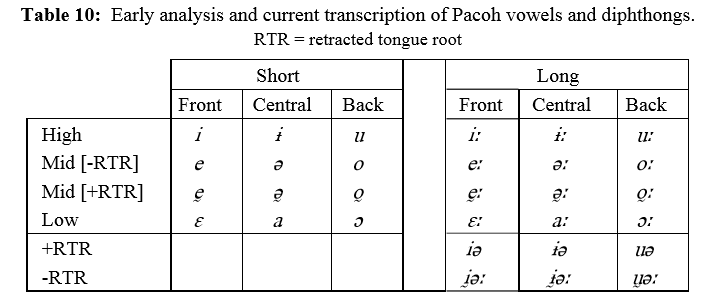
\includegraphics[width=\linewidth]{Pacoh/src/PacohTable10.png}
\end{center}

\item 2가지 높이(고저) 분류. 모든 모음에 대해 혀뿌리 위치 후진 여부(retracted/nonretracted)에 따라 하위 그룹을 상정하는 방식. = registers system. R. Watson 은 1980년 이후부터 고려하기 시작.
\begin{center}
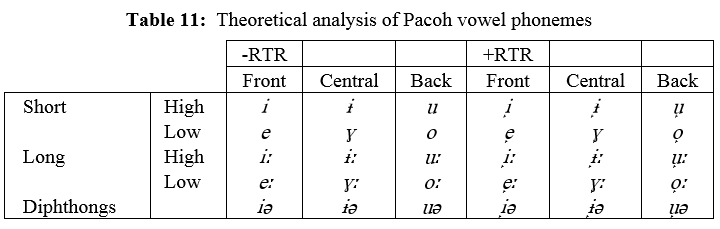
\includegraphics[width=\linewidth]{Pacoh/src/PacohTable11.png}
\end{center}
\end{enumerate}

\item Alves(2000)는 두번째 방식을 유표적(marked)으로 보는 동시에 몇 음소에 대해서는 음소-음성 간 불균형이 너무 심하다고 보지만 전반적인 음소적 균형과 몬·크메르어의 register 체계와 유형론적으로 맞다는 이론적인 관점에서 Watson의 이후 입장(=두번째 방식)을 합리적인 것으로 평가한다.

\item 음소의 개수는 변하지 않는다. 빠꼬어에는 24개의 단모음, 6개의 이중모음이 있다. 표11의 마지막 두 줄은 현재 방식의 음운론적 분석에 따르면 모두 +RTR이다. 표11에서 나타나는 것은 음운론적 분석 상 선호되는 것이고, Alves(2000)와 저자는 표10에서와 같이 음성적 실현음에 맞추어 전사한다.
\end{itemize}

\subsubsection{모음 장단}
\begin{itemize}
\item 모음의 장단은 모음 자질(quality)에 큰 영향 없음. (e.g. 장모음은 이중모음화하지 않음.)

\item 그러나 음운적으로 유의미한 차이. 최소대립쌍 존재.

\item 장모음은 개음절과 폐음절에 모두 나타나고 단모음은 폐음절에만 나타남. 음성적인 지속 길이의 비율은 높은 경우 1.5 대 1. (150 대 100 m/s)
\end{itemize}

\subsubsection{Register의 변화:  [+RTR] 모음}
몬·크메르어파 언어의 음운론에서는 `register'이라는 자질에 의해 모음의 목록이 두 배가 된다. 무표적인 평 모음 (`clear vowels')에 대비되는, 기식음(breathiness), 짜내는 소리(creakiness), 거친 소리(raspiness) 등 주로 phonation의 차이를 보이는 모음들을 변화된 register를 갖춘 모음이라고 부르는 것이다(Matisoff 1973; Gregerson 1976). 유표적인 register를 갖춘 모음들은 역사적으로 계속 변화하기 때문에, 어떤 몬·크메르어파 언어에서는 R. Watson(1996)이 지적했듯이 register상 평 모음과 유표적인 모음이 병합되기도 했다.

빠꼬어에서는 RTR(`retracted tongue root', 혀뿌리의 후진)이라는 음성적 자질을 통해 이러한 유표적인 모음을 기술한다. 빠꼬어 모음에서 혀뿌리가 후진되면 결과적으로는 거친 소리(raspy sound)가 나타난다. 빠꼬어 단어에서 이러한 모음에는 분포 상 제약이 따른다. [+RTR] 모음은 주 음절에만 나타나고 전음절에는 나타나지 않는다. 몬·크메르어의 전음절에는 애초에 허용되는 모음의 수가 적은 편이다. 어떤 언어에서는 슈와(schwa)만이 허용되기도 한다. 빠꼬어와 다른 몇몇 Katuic 언어들에서는 [i], [a], [u]의 세 소리만 허용된다.

가장 특기할 만한 것은 +RTR 모음이 -RTR 대응 모음보다 음성적으로 저모음이며 더 높은 F1이 나타난다는 사실이다.

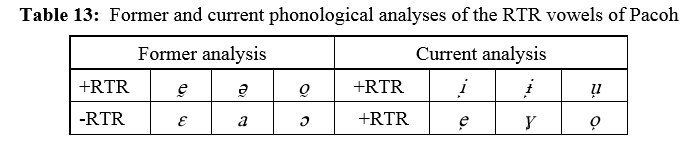
\includegraphics{Pacoh/src/PacohTable13.png}

(기존에 -RTR로 분류하던 모음들도 포함해서) 6개의 기본 [+RTR] 모음은 그 상대음(counterpart)와는 명확히 다르다.
/i̙/는 성문음화된 [ḛ]로 실현, /ɤ̙/는 [a]로 저모음화, /u̙/는 성문음화된 [o̰]로 실현, /e̙/는 [ɛ]로 저모음화, /ɨ̙/는 성문음화된 슈와 [ə̰]처럼 들리고 /o̙/는 [ɔ]로 저모음화.
(이전에 -RTR로 분류하던 모음들도 저모음화하므로 +RTR로 분류하는 게 타당하다는 말인 듯)

\subsubsection{이중모음}
이중모음은 장모음이고 열린 단음절과 주음절에 모두 올 수 있다. 음성적으로 이중모음은 다른 장모음보다 15m/s정도 길게 지속된다. 뒷부분의 경과음(final off-glides)는 슈와 기호로 전사했는데, 실제 음성적 실현음은 이중모음의 최고점(peak) 위치에 따라 다르다. 기본 이중모음 세 가지는 RTR 자질에 의해 두 그룹(classes)으로 나뉜다.

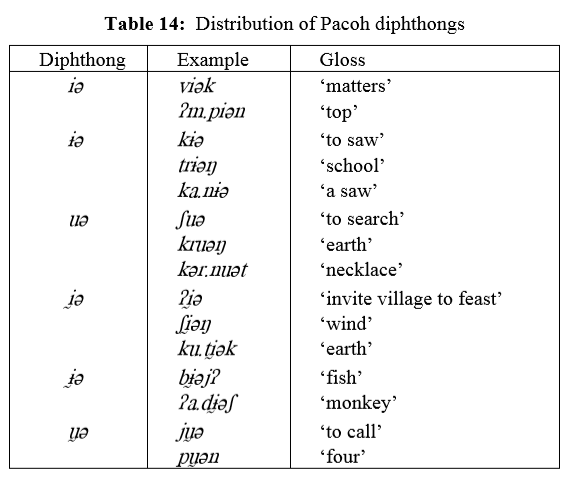
\includegraphics{Pacoh/src/PacohTable14.png}

\subsection{음운론적 단어와 음절의 구조}
빠꼬어에서 \textbf{통사적 단어(syntactic word)}에 대해서는 음운론적 제한이 없어 하나의 의미적 개념에 대해 긴 음절 연속이 가능한 데 반해,  \textbf{음운론적 단어(phonological word)}의 음절 갯수는 2개로 제한된다. 
음운론적 단어에는 주 강세(main stress)가 하나만 존재하지만, 통사적 단어에서는 하나 이상이 나타날 수 있다. 반복어(reduplicants)와 일부 단음절어에서 파생된 어휘적 합성어들은 단음절들로 구성되지만 강세의 정도가 두 음절에서 동일하므로 2개의 음운론적 단어로 구성된다고 할 수 있다. 통사적 단어 하나를 구성하는 음운론적 단어들은 하이픈으로 분지하고(이는 형태소를 분지하는 것이 아니고 연결된 음운론적 단어를 강조하고자 하는 것이다.), 음운론적 단어 안에서 나타나는 음절들은 온점으로 분지한다. \\

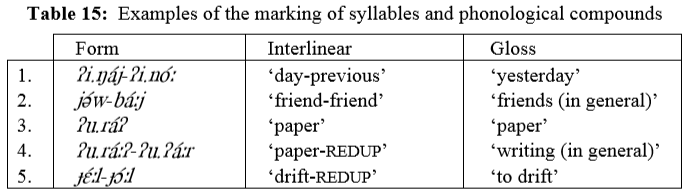
\includegraphics{Pacoh/src/PacohTable15.png}

1번과 2번에서 자립적인 형태(free forms)가 결합하여 만들어진 통사적 단어의 예를 볼 수 있다.
1번 예시를 다수의 어휘가 결합된 것이 아니라 하나의 어휘로 보는 근거는 /ʔi.noː/라는 형태가 별개 어휘로 나타나지 않기 때문이고, 2번 예시를 하나의 어휘로 보는 근거는 두 음절의 순서가 서로 바뀔 수 없기 때문이다.
4번과 5번은 반복을 통한 어휘 형성이다. 강세는 예측 가능하기 때문에 이 문법서에서는 표기하지 않지만, 여기서는 각 음운론적 단어에 강세가 모두 표시되어 있다. 모든 음운론적 단어는 마지막 음절에 하나의 강세를 갖는다.

음운론적 단어의 층위 위에는 \textbf{음운론적 구(phonological phrase)}라는 층위가 있다. 음운론적 구에서는 주 강세가 하나 나타나고, 하나 또는 여러 개의 음운론적 단어가 나타날 수 있다. 빠꼬어의 음운론적 단어는 2음절 이하이기 때문에 언제나 하나의 운율론적 음보(prosodic foot)에 대응되고 따라서 단어와 음보(feet)는 공존한다. 빠꼬어는 강약(trochaic) 모라(mora) 음보를 갖추고 있고, 음보를 벗어나는 (unfooted) 모라 하나가 왼쪽에 나타날 수 있다.
빠꼬어의 음운론적 단어는 하나 또는 두 개의 음절로 구성된다. 한 음절은 강세에 따라 하나 또는 두 개의 모라로 구성된다. 강세를 받은 음절은 모라가 2개이고(bimoraic) 강세를 받지 않는 음절은 모라가 1개이다(monomoraic). 모라 중량 요구(moraic weight requirements)는 주로 모음이 충족시키지만 자음 또한 충족시킬 수 있다.

\subsubsection{전반적 음절과 단어의 구성}
모든 빠꼬어 음운론적 단어에서 주음절은 필수, 전음절은 선택적. 모든 음절은 공명음 핵(모음, 비음 또는 유음)을 갖춰야 하고 음절초 자음을 갖추어야 함(성문 폐쇄음 포함).

\textbf{주음절} 음절초에서는 단자음과 자음군이 모두 나타날 수 있음. 빠꼬어 고유어에서 자음군의 두 번째 분절음은 [l] 또는 [r]. 베트남어 차용어에서는 활음([j]또는 [w])이 나타날 수 있음. 주음절은 강세를 갖추어야 하고 모라는 반드시 두 개. 모라 중량 요구는 장모음이나 모음+음절말 자음의 조합으로 충족시킬 수 있음. 주음절은 홀로, 또는 이차적인 전음절과 함께, 또는 (반복어에서) 다른 주음절과 함께 발음될 수 있음.

\begin{center}
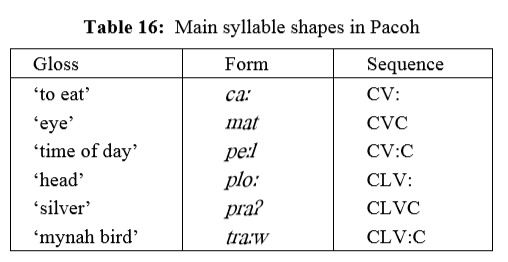
\includegraphics{Pacoh/src/PacohTable16.png}
\end{center}

\textbf{전음절}은 형태, 중량, 강세와 분포가 다양함. 모든 빠꼬어 전음절은 최소한 하나의 음절초 자음과 공명음 정점(peak)을 갖춤. 그러나 자음군은 허용되지 않고 모음은 언제나 단모음. 언제나 강세를 받지 않고 하나의 모라만을 받음. 독특한 점 한 가지는 빠꼬어 전음절의 공명음 정점이 비음이나 유음도 허용한다는 것. 전음절이 개음절일 경우 /i/, /a/, /u/ 만을, 폐음절일 경우 /ə/만을 허용하고 음절 말음은 언제나 유음이나 비음이다.
표17의 세 번째 예시에서처럼 공명음이 핵으로 나타나는 경우 언제나 앞에 음운론적으로 변별적이지 않은 성문 폐쇄음이 나타난다.

\begin{center}
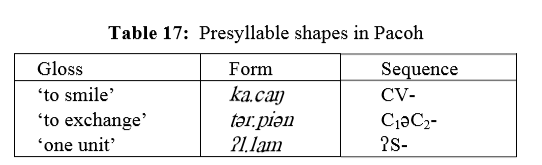
\includegraphics{Pacoh/src/PacohTable17.png}

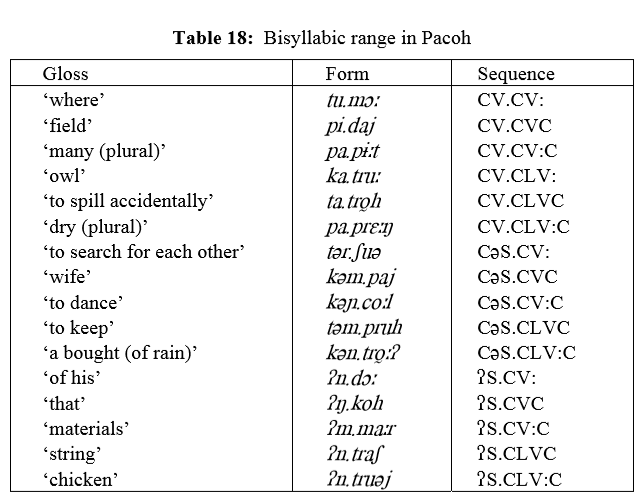
\includegraphics{Pacoh/src/PacohTable18.png}
\end{center}

유일하게 CəS.CLV: 에 대해서는 사례를 발견하지 못하였다.

\subsubsection{운율론적 제약}
모든 빠꼬어 음절은 자음으로 시작해야 하고 공명음 정점(a sonorant peak)이 있어야 한다. 공명음 정점은 모음이 될 수 있고, 특별히 전음절에서는 비음이나 유음이 될 수 있다. 빠꼬어 전음절은 CV, CVS 또는 CS의 조합을 갖출 수 있고, 주음절은 CV:, CVC, CV:C의 조합을 갖출 수 있다. 전음절의 정점이 되는 공명음(비음, 유음)에는 언제나 성문 폐쇄음이 선행하고 다른 자음은 앞에 올 수 없다. 열린 전음절에는 /i/, /a/, /u/가 나타나지만 닫힌 전음절(checked syllables)에는 슈와만이 나타난다.

빠꼬어에서 강세를 받는 모든 음절(단음절 단어, 또는 이음절 단어의 두 번째 음절)은 2개의 모라를 갖춘다. 강세 없는 음절은 1모라. 하나의 모라는 (전음절 또는 주음절의) 단모음이나 비음 핵을 갖는 전음절에 대응된다. 한 쌍의 모라는 장모음, 이중모음, 그리고 단모음과 음절말 자음의 조합에 대응된다. 장모음이나 이중모음을 갖춘 음절의 마지막 자음에는 모라 중량이 할당되지 않는다. 이러한 제약에 의해 전음절에는 음절말 자음이 있든 없든 언제나 하나의 모라만이 할당된다. 언제나 강세를 갖는 주음절에는 언제나 두 개의 모라가 할당된다.

\begin{center}
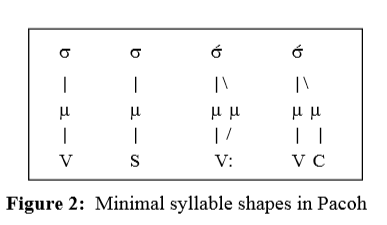
\includegraphics{Pacoh/src/PacohFigure2.png}
\end{center}

VC 조합에서는 장모음과 단모음 모두 나타날 수 있지만 장모음이 나타나는 경우엔 두 모라 중량에 모두 장모음이 기여한다. (음절말 자음의 분량은 없다)

빠꼬어의 음운론적 단어는 전부 두 가지로 나뉜다: 강세가 있는 단음절 단어, 마지막에 강세가 있는 2음절 단어. 강세를 받는 음절은 더 길고 크게 발음된다.

형태음운론적 과정상 이음절어에 대한 선호(이음절어로 축약하도록 만드는 압력)가 나타남.
예를 들어 [ku.mɔː] `year' 과 수사 [ʃoːŋ] `five'가 만나면 [ku.mɔː.ku.moːŋ]이 아닌 [ku.moːŋ]이 됨. [ku.mɔː-ku.moːŋ] 은 `five years from now' 이고, 이것은 [ku.mɔː]에만 특정적인 수식. (아마도 [ku.mɔːʃoːŋ]이라는 형태를 가정하지 않는 데 대한 설명인 듯)

\begin{center}
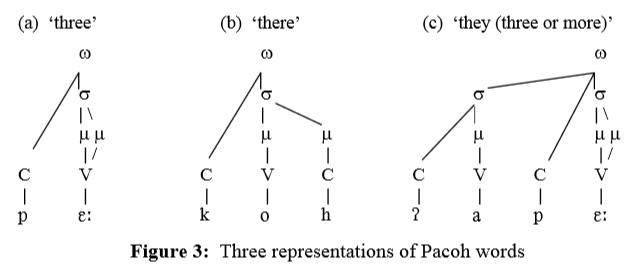
\includegraphics{Pacoh/src/PacohFigure3.png}
\end{center}

\subsubsection{음소배열론적 제약}
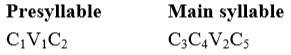
\includegraphics{Pacoh/src/Pacohsyllablestructure.png}

C1은 후-성문음화된 활음이나 유기 폐쇄음을 제외하고 모든 자음이 올 수 있다. C2에는 활음을 제외한 공명음, 즉 비음과 유음만이 올 수 있다. C3은 후-성문음화된 활음을 제외한 모든 자음이 올 수 있다. 그러나 유음을 선행하는 경우 /p/, /t/, /k/로 제한. C4는 자음군의 유음 /r/과 /l/만이 허용된다. C5는 유성폐쇄음과 유기폐쇄음을 제외한 모든 자음이 허용된다. C5는 장모음 뒤에는 선택적으로 나타나지만 단모음 뒤에는 필수적으로 나타난다.

빠꼬어에서는 음절 정점으로 갈수록 공명성이 증가. 공명도는 낮은 쪽부터 장해음, 비음, 유음, 활음, 모음 순. 고유 어휘에는 자음군의 둘째 자리에 활음이 나타나지 않지만, 베트남어 차용어에는 나타난다. 해당 위치에서 활음에 대한 제약이 없다는 뜻. 공명도 제약에도 부합함.

후-성문음화된 폐쇄음의 출현도 공명도 제약을 고려할 때 합리적이다. 공명도가 높았다가 낮아지므로 음절 말 위치에는 적합하고 음절초 위치에는 적합하지 않은 것이다.

전음절에는 [+RTR] 모음 없음. 

전음절은 분절음적으로도 운율론적으로도 주음절에 의존적. 비음의 조음점 동화, 음절초 자음 동화.

\subsubsection{공명음 전음절: 비음과 유음}
음절 구조 제약(늘 첫 소리가 자음일 것)에 의해 항상 성문 폐쇄음이 삽입됨.

전음절 비음은 주음절 첫 자음에 조음 위치가 동화됨.

비음 음절에 모음이 완전히 없다는 음성학적 증거. 제2포먼트 주파수가 관찰되지 않고 모음을 갖춘 전음절보다 강도가 상대적으로 낮음.

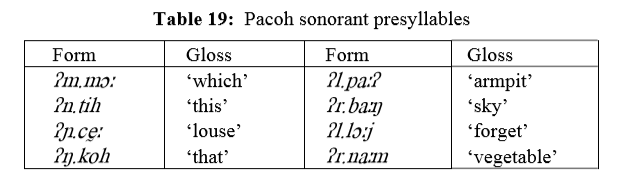
\includegraphics{Pacoh/src/PacohTable19.png}

\subsubsection{자음군}
[kl], [kr], [pl], [pr], [tr]의 다섯 가지. Watsons와 ND\&P에서는 모두 [pʰ] [tʰ] [kʰ]를 자음군 음소로 보았다. (즉 /p/+/h/ 등)

R. Watson(1964) 접요사를 삽입하는 형태음운론적 실험.
kʰiər `마당을 쓸다' ka.niər `마당 빗자루' [h] 소실. 이러한 삽입은 요즘은 잘 일어나지 않고 몇몇 단어에만 남아있지만 유기음을 두 음소의 결합으로 보는 근거.

동남아의 유형론적인 경향성인 음절초 자음군 단순화의 하나로 볼 수 있음. 이 지역 다른 언어들에도 나타났고 나타나는 중인 현상.

\subsection{반복어}
\begin{enumerate}
\item 견본(template): 완전 반복, 일부 교체
\item 전음절(presyllabic)
\item 부분적
\item 견본-접사(template-plus-affix)
\end{enumerate}

빠꼬어에서 가장 흔한 유형은 견본과 음절초 자음 반복.

\textbf{견본} 반복에서는 음운론적 단어 하나의 모든 운율이 베껴짐. 그대로 베껴질 수도 있지만, 모음, 자음, 음절의 운(rhyme, 모음과 음절말 자음, 즉 음절의 1모라 부분) 중 하나는 교체될 수 있음.

\textbf{견본-접사} 반복에서는 (1) 음절 하나가 통째로 반복되고 [ʔi] 또는 [ʔm]라는 음절이 두 음절 사이에 끼거나 (2) 주음절의 첫소리가 전음절의 첫소리로 베껴진다.

두 경우 모두 단음절 단어나 이음절 단어를 기반으로 반복어를 만든다.

\begin{center}
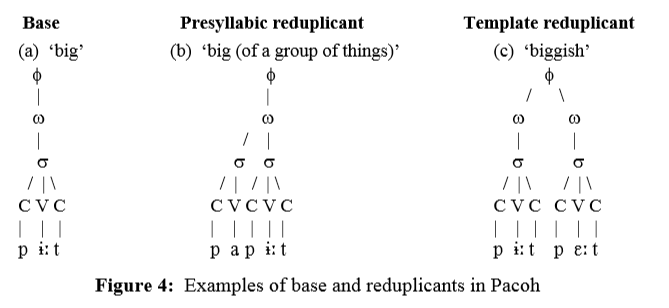
\includegraphics{Pacoh/src/PacohFigure4.png}
\end{center}

(b)에서는 전음절 반복어(presyllabic reduplicant)를 형성하기 위해 주음절의 첫 자음이 베껴졌고 접두사를 만들기 위해 /a/가 삽입되었다. (c)에서는 음절 견본 전체가 베껴졌지만 일부 분절음(이 경우에는 모음)이 교체되었다.

\subsubsection{견본 반복}
운율론적 견본 반복에서 반복어는 분절적으로 정의되지 않은 음절이고 그것을 원어의 분절음이 채운다.

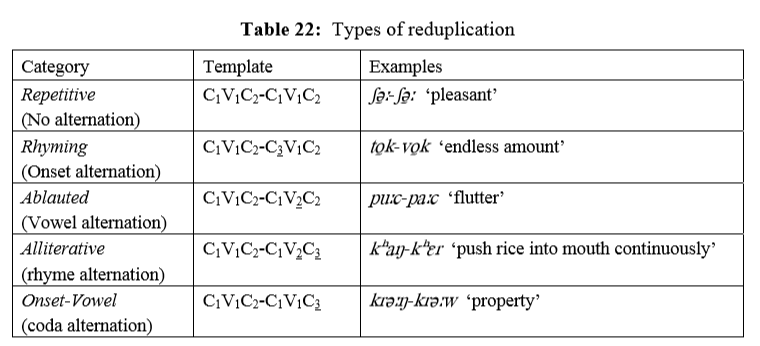
\includegraphics{Pacoh/src/PacohTable22.png}

교체된 음소에 밑줄. (크메르어에도 유사한 현상 나타남.)

완전반복(교체 없음)은 가장 드문 경우. 

교체되는 분절음은 운율론적 기능 상 원어의 분절음과 대응된다. (원어에서 자음이 나타난 위치에는 반복어에서도 자음이 나타나고, 모음이 나타난 위치에는 모음이 나타남)

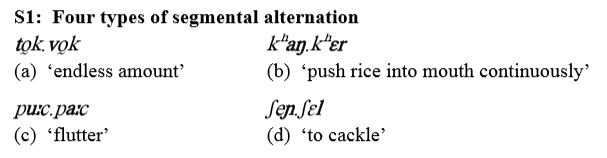
\includegraphics{Pacoh/src/PacohS1.png}

교체된 분절음에 볼드 처리. 음절초 자음과 모음의 조합이 교체되거나 모음은 그대로고 두 자음이 모두 교체되는 경우는 관찰되지 않는다.

\subsubsection{음절초 자음 반복}
음절초 자음 반복에서는 원어의 음절초 자음이 복사되고 [a]가 삽입된다. 이러한 전음절의 예들은 모두 다음절이 아닌 단음절 형태를 기반으로 형성된다. 도식4의 `크다' 참조. 전음절의 음절 첫소리는 정의되지 않은 상태이고(unspecified) 원어에서 채워진다. 모음은 [a].

\subsubsection{부분적 반복}
이음절인 원어의 주음절 하나를 분절음 교체 없이 완전히 반복하여 따라붙음. 

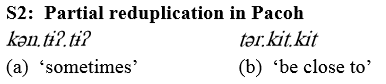
\includegraphics{Pacoh/src/PacohS2.png}

\subsubsection{접요사와 견본 반복}
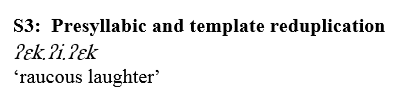
\includegraphics{Pacoh/src/PacohS3.png}

완전 반복, 두 음절 사이 비-반복적인 /-i-/ 삽입.

\subsection{억양}
개별 단어의 어휘 강세(lexical stress)를 넘어서는 구의 주 강세(primary phrasal stress)가 억양의 단위를 만들어낸다.

빠꼬어는 주로 모라mora-timed 언어. 2음절 단어의 두 번째 음절은 2모라, 음성적으로 더 두드러짐(prominent). 따라서 음운론적 구에서 억양 정점(intonational peaks)을 만들어내는 경향이 있는 강세음절을 갖춘 이음절 단어가 구의 억양을 어느정도 조건지을 수 있음. 그러나 발화의 내용과 기능어가 더 중요한 요소.

문법적 기능을 나타내는 단어(grammatically functional words)에서보다 내용을 나타내는 단어(content words)에서 억양은 더 두드러진다.

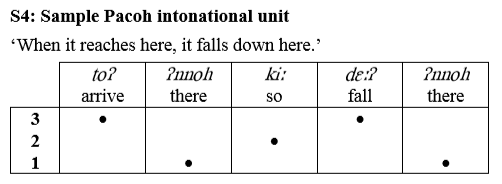
\includegraphics{Pacoh/src/PacohS4.png}

의문문 억양은 올라가고 비-의문문 억양은 내려간다. 의문조사(interrogative sentence particle)이 있음에도 억양의 상승은 필수적이다. 

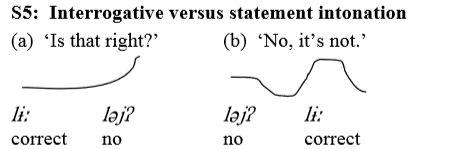
\includegraphics{Pacoh/src/PacohS5.png}

S5a에서 억양 상승이 요구된다. 두 단어의 크기(loudness)는 비슷하다.

\subsection{차용어 음운론}
베트남어는 성조어. 성조는 받아들이지 않았으나 일부 성조의 성문음화는 받아들임. 그래서 후-성문음화된 비음이 생겼음. 빠꼬어 고유 어휘에는 후-성문음화된 활음만이 존재하지만 비음의 후-성문음화를 막을 어떤 음운론적 제약이 존재하지 않는다는 것을 보여줌.

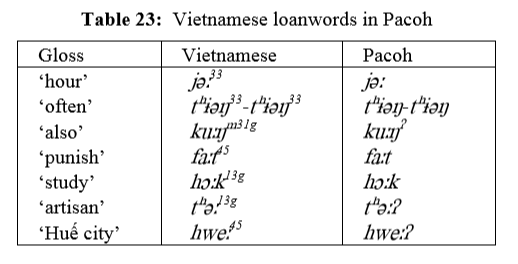
\includegraphics{Pacoh/src/PacohTable23.png}

베트남어에서 5는 고조, 1은 저조. g는 성문음화를 나타냄. 후에 시의 이름에서 빠꼬어 고유어에서와 다르게 활음이 들어간 자음군이 허용되는 것을 관찰할 수 있음.
